\documentclass{article}
\usepackage{pgfplots}
\pgfplotsset{compat=1.16} % Use the required version of pgfplots

\begin{document}

\begin{figure}[h]
    \centering
    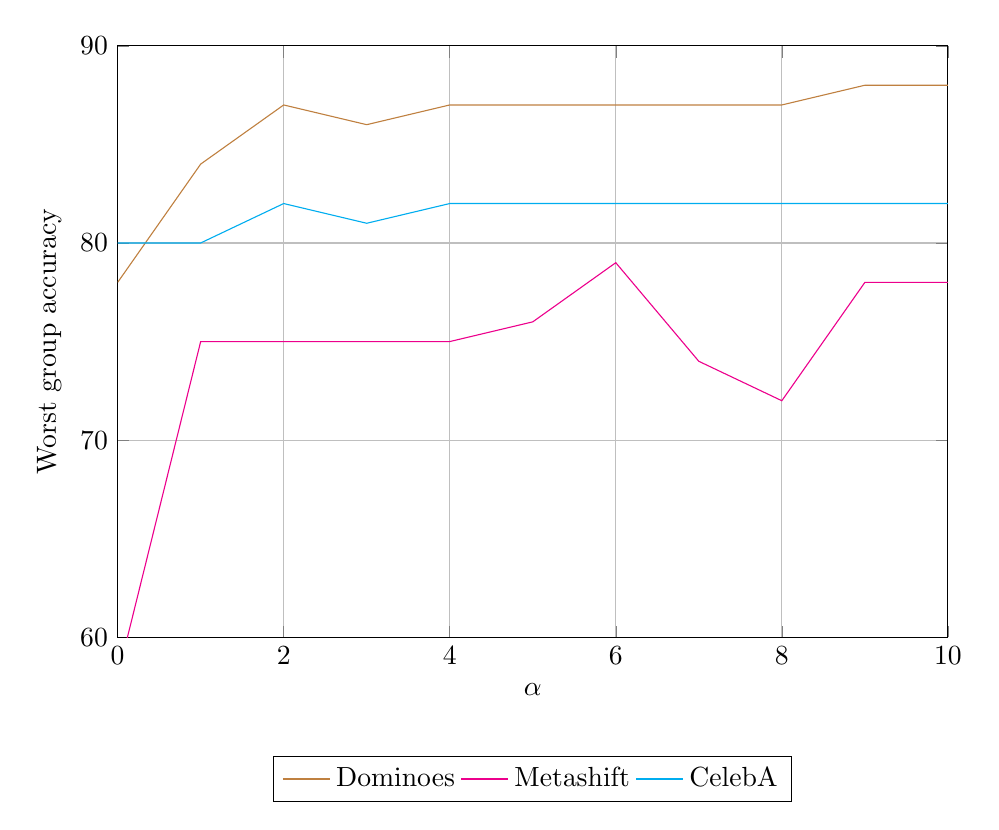
\begin{tikzpicture}
        \begin{axis}[
            width=\textwidth,
            height=0.75\textwidth,
            xlabel={$\alpha$},
            ylabel={Worst group accuracy},
            legend style={at={(0.5,-0.2)},anchor=north,legend columns=-1},
            grid=both,
            xmin=0, xmax=10,
            ymin=60, ymax=90,
            xtick={0,2,4,6,8,10},
            ytick={60,70,80,90},
            ]
            
            \addplot [
                color=brown,
                mark=none,
                ]
                coordinates {
                    (0,78) (1,84) (2,87) (3,86) (4,87) (5,87) (6,87) (7,87) (8,87) (9,88) (10,88)
                };
                \addlegendentry{Dominoes};
                
            \addplot [
                color=magenta,
                mark=none,
                ]
                coordinates {
                    (0,58) (1,75) (2,75) (3,75) (4,75) (5,76) (6,79) (7,74) (8,72) (9,78) (10,78)
                };
                \addlegendentry{Metashift};
                
            \addplot [
                color=cyan,
                mark=none,
                ]
                coordinates {
                    (0,80) (1,80) (2,82) (3,81) (4,82) (5,82) (6,82) (7,82) (8,82) (9,82) (10,82)
                };
                \addlegendentry{CelebA};
                
        \end{axis}
    \end{tikzpicture}
    
    \caption{Worst group accuracy on different datasets with respect to $\alpha$. $\alpha\geq 1$ is enough to increase worst group accuracy rapidly.}
    \label{fig:worst_group_accuracy}
\end{figure}

\end{document}